\documentclass[a4paper]{article}

%% Language and font encodings
\usepackage[english]{babel}
\usepackage[utf8x]{inputenc}
\usepackage[T1]{fontenc}

%% Sets page size and margins
\usepackage[a4paper,top=3cm,bottom=2cm,left=3cm,right=3cm,marginparwidth=1.75cm]{geometry}

%% Useful packages
\usepackage{amsmath}
\usepackage{graphicx}
\usepackage[colorinlistoftodos]{todonotes}
\usepackage[colorlinks=true, allcolors=blue]{hyperref}
\usepackage{amsfonts}

\title{Digital Signal Processing - week5 quiz solutions}


\begin{document}
\maketitle

\section{Question 1}
Which of the following are linear systems:

\subsection{} 
\begin{enumerate}
\item Envelope detection (via squaring), i.e. $y[n] = \vert[n]\vert^2 \ast h[n]$
 where h[n] is the impulse response of a lowpass filter such as the moving average filter.
\item This is obviously not liner since squaring is not linear
\end{enumerate}

\subsection{}
\begin{enumerate}
\item AM radio modulation, i.e. multiply a signal x[n] by a cosine at the carrier frequency :
$y[n]= x[n]\cos(2\pi\omega_cn)$
\item It is linear:  $(ax_1[n]+bx_2[n])\cos(2\pi\omega_cn) = ax_1[n]\cos(2\pi\omega_cn)+bx_2[n]\cos(2\pi\omega_cn) = ay_1[n]+by_2[n]$
\end{enumerate}

\subsection{}
\begin{enumerate}
\item Second derivative, i.e. $y(t) = \frac{d^2}{dt^2}x(t)$
\item It is easy to see that derivative operation is linear
\end{enumerate}

\subsection{}
\begin{enumerate}
\item Clipping, i.e. enforce a maximum signal amplitude MM,e.g: 
$$
y[n] = \begin{cases} x[n] &\mbox{if } x[n] \leq M  \\
M & \mbox{otherwise } \end{cases} 
$$
\item take $x_1[n]=x_2[n] =M+1$ then $x_3[n] = x_1[n]+x_2[n] = 2M+2$ but $y_1[n]=y_2[n] = y_3[n] = M$
So $y_3[n] \ne y_1[n] + y_2[n]$
\end{enumerate}

\section{Question 5}
\subsection{Q}


Consider the filter $h[n]=\delta[n]-\delta[n-1]$, and the input $x[n] = \begin{cases} n &\mbox{if } n \leq 0  \\
0 & \mbox{otherwise } \end{cases}$ 

and the output $y[n]=x[n]\ast h[n]$.

Compute $y[-1],y[0],y[1],y[2]$

\subsection{A}
$y[n]=x[n]\ast h[n] = x[n]\ast (\delta[n]-\delta[n-1]) = x[n]\ast \delta[n] - x[n]\ast \delta[n-1] = x[n] - x[n-1] $. Therefore:
\begin{enumerate}
\item $y[-1] = x[-1] - x[-2] = 0$
\item $y[0] = x[0] - x[-1] = 0$
\item $y[1] = x[1] - x[0] = 1$
\item $y[2] = x[2] - x[1] = 1$
\end{enumerate}

\section{Question 6}
\subsection{Q}
Which of the following filters are BIBO-stable?
Assume $N \in \mathbb{N}$ and $0 < \omega < \pi$
 
\subsection{A}
\begin{enumerate}
\item Any filter $h[n]$ with finite support and bounded coefficients.
Is BIBO-stable - it is absolutly summable
\item the moving avarage. Is BIBO stable - if the input is bounded so is the output.
\item The following smoothing filter: $h[n]=\sum_{k=0}^\infty \frac{1}{k+1}\delta[n-k]$.
is NOT BIBO-stable - this is the harmonic series which is not absolutly summble.
\item The ideal low pass filter with a cutoff frequency $\omega$:

$$
H(e^{j\omega}) = \begin{cases} 1 &\mbox{if } |\omega| \leq \omega_c  \\
0 & \mbox{otherwise } \end{cases} 
$$
is NOT BIBO stable since $sinc$ is not absolutly summble.
\end{enumerate} 

\section{Question 7}
\begin{figure}
\centering
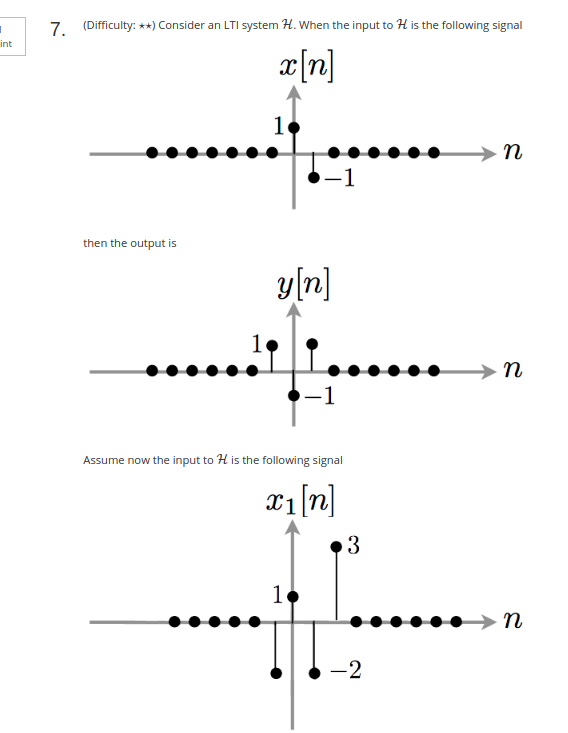
\includegraphics[width=0.7\textwidth]{week5_q7.png}
\caption{\label{week5_q7}Question 7}
\end{figure}

\subsection{Q}
See the figure for question 7.
\subsection{A}
We need to find the impules response $h[n]$ from the given input and output.
$$
y[n] = x[n] \ast h[n] = \Sigma x[k]h[n-k] = x[0]h[n] + x[1]h[n-1] = 1h[n] +(-1)h[n-1] = h[n] - h[n-1]
$$

\begin{enumerate}
\item for $n \leq -2 , n \geq 2$ we have $y[n] = h[n] - h[n-1] = 0$ so $h[n] = h[n-1]$
\item for $n=-1$:  $y[-1] = h[-1] - h[-2] = 1 \rightarrow h[-1] = h[-2] + 1$
\item for $n=0$:  $y[0] = h[0] - h[-1] = -1 \rightarrow h[0] = h[-1] - 1 = h[-2] + 1 - 1 = h[-2]$
\item for $n=1$:  $y[1] = h[1] - h[0] = 1 \rightarrow h[1] = h[0] + 1 = h[-2] + 1$
\end{enumerate}
define $A := h[-2]$ so $h[-1] = A+1$, $h[0] = A$, $h[1] = A + 1$.

So $h[n]$ looks: $... A, (A)_{-2}, (A+1)_{-1}, (A)_{0}, (A+1)_{1}, (A+1)_{2}, ...$. 

Now we have $x_1[n]= .. 0,0,-2_{-1},1_{0},-2_{1},3_{2},0,0, ..$ so:
\begin{enumerate}
\item 
$$
y_1[-2] = (x_1[n] \ast h[n])(-2) = \Sigma x_1[k]h[-2-k] = x_1[-1]h[-1] + x_1[0]h[-2] + x_1[1]h[-3]+x_1[2]h[-4]
$$
$$
 = -2(A+1) + (1A) + (-2A)+(3A) = -2
$$
\item 
$$
y_1[-1] = (x_1[n] \ast h[n])(-1) = \Sigma x_1[k]h[-1-k] = x_1[-1]h[0] + x_1[0]h[-1] + x_1[1]h[-2]+x_1[2]h[-3]
$$
$$
 = (-2A) + 1(A+1) + (-2A)+3A = 1
$$
\end{enumerate}

\section{Question 12}
 \begin{figure}
\centering
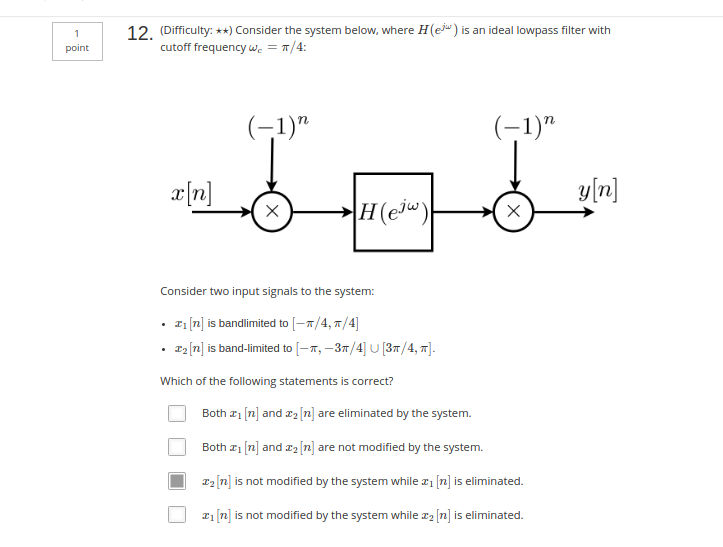
\includegraphics[width=1\textwidth]{week5_q12.png}
\caption{\label{week5_q12}Question 12}
\end{figure}

\subsection{Q}
See the figure for question 12.

\subsection{A}
The way to solve it is to note that $(-1)^n = \cos(\pi n)$ so multiply by $(-1)^n$ is 
equivalent to modultation with $\omega_0 = \pi$.

From week 4 we know $DTFT\{x[n]cos(\omega_0 n)\} = \frac{1}{2}(X(e^{j(\omega-\omega_0)}) +  X(e^{j(\omega+\omega_0)}) )$.

Also, one should remember the $2\pi$ preiodicity, from there it is easy to note that the system eliminates 
$x_1$ and does not modify $x_2$


\section{Question 14}
 \begin{figure}
\centering
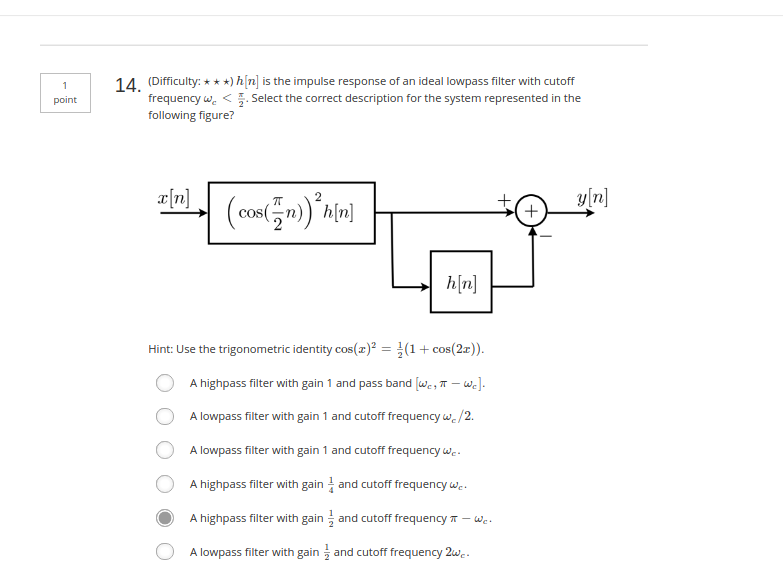
\includegraphics[width=1\textwidth]{week5_q14.png}
\caption{\label{week5_q14}Question 14}
\end{figure}

\subsection{Q}
See the figure for question 14.

\subsection{A}
The thing to note here is that the $\cos(\frac{\pi}{2}n)^2$ and the $h[n]$ are not convulated but
multiplyed, so it relates to modulation of the $h[n]$ filter.

From the hint we have $\cos(\frac{\pi}{2}n)^2 = \frac{1}{2}(1+\cos(\pi n))$ and we have from modulation:
$$
DTFT\{\frac{1}{2}(1+\cos(\pi n))h[n]\} = \frac{1}{2}DTFT\{h[n]\} + \frac{1}{4}(H(e^{j(\omega-\pi)}) +  H(e^{j(\omega+\pi)}) )
$$
$$
= \frac{1}{2}H(e^{j\omega}) + \frac{1}{4}(H(e^{j(\omega-\pi)}) +  H(e^{j(\omega+\pi)}) )
$$
So the system in the frequency domain is:
$$
X(e^{j\omega})(\frac{1}{2}H(e^{j\omega}) + \frac{1}{4}(H(e^{j(\omega-\pi)}) +  H(e^{j(\omega+\pi)}) )(1-H(e^{j\omega}))
$$

First we multiply with a filter that take the low frequencies and the high frequencies, so we
eliminate the bandpass frequencies.
Then we multiply with a highpass filter, so overall the final system is a highpass filter.
Note that because of perudicity, the high frequencies is a sum of the modulation from $0 \rightarrow \pi$ and
from $\pi \leftarrow 2\pi$ and since it is multiplied by $\frac{1}{4}$ the overall gain is $\frac{1}{2}$.

\section{Question 15}
 \begin{figure}
\centering
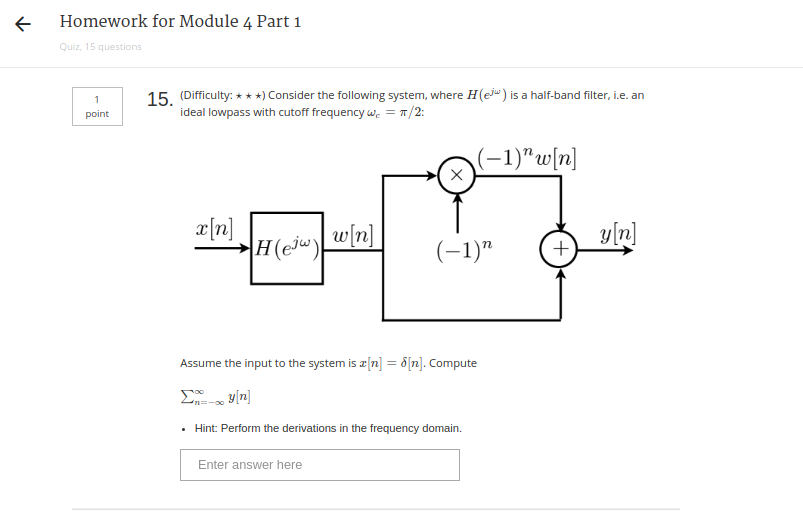
\includegraphics[width=1\textwidth]{week5_q15.png}
\caption{\label{week5_q15}Question 15}
\end{figure}

\subsection{Q}
See the figure for question 15.

\subsection{A}
Since $x[n] = \delta[n]$ then $y[n]$ is the system itself. Note again that multiplying by $(-1)^n$
is a modulation with $\cos(\pi n)$ so the system is the sum of the filter $h[n]$ and it's modulation with
$\cos(\pi n)$ but $h[n]$ is a lowpass filter with cutoff freq $\frac{\pi}{2}$ so the system in the frequency sapce (call it $S(e^{j\omega})$) is $S(e^{j\omega}) = 1$ for each $\omega$ (the sum of $H$ and it's modulation covers the whole range).


Now, note that $\Sigma y[n] = (y[k]\ast 1)[0]$. So in the frequency domain it is $S(e^{j\omega}) DTFT\{1\}$.
Also $DTFT\{1\}$ is an impulse train with period $2\pi$ and amplitude $2\pi$.

So we have:
$$
\Sigma y[n] = (y[k]\ast 1)[0] = \frac{1}{2\pi} \int_{-\pi}^{\pi}S(e^{j\omega}) DTFT\{1\}e^{j\omega 0}d\omega = \frac{1}{2\pi} \int_{-\pi}^{\pi}DTFT\{1\}d\omega = \frac{1}{2\pi} \int_{-\pi}^{\pi}2\pi\delta(\omega)d\omega = 1
$$

\end{document}
